\documentclass[a4paper, titlepage]{jsarticle}

\usepackage[utf8]{inputenc}

\usepackage[dvipdfmx]{graphicx}
\usepackage[dvipdfmx]{xcolor}

\usepackage{hyperref}
\usepackage{mathtools}
\usepackage{tikz}
\usepackage{amsmath}
\usepackage{amssymb}
\usepackage{amsfonts}
\usepackage{latexsym}
\usepackage{enumitem}
\usepackage{empheq}
\usepackage{amsthm}
\usepackage{bm}
\usepackage{physics}

\usetikzlibrary{
   positioning,
   arrows.meta,
   graphs
}

\title{\Huge スパイキングニューラルネットワークについて}
\author{\Large 創域理工学部\quad 情報計算科学科\quad 4年\\\Large 学籍番号\;:\;6322045\\\Large 砂川恵太朗}
\date{提出日\;:\;\today}

\begin{document}

\maketitle

\section{この資料の位置づけについて}
Spiking neural network(SNN)は,その他のニューラルネットワークと同様に,エンコーダ・ニューロンモデル・デコーダ・学習則の要素がある.SNNには様々なモデルがあるが,各要素に対してそれぞれのモデルからかいつまんで説明するのは,各要素同士のつながりが欠けてしまうので,ここでは最もポピュラーとされるDiehl\&Cookモデルを紹介しようと思う.以下,論文"Unsupervised learning of digit recognition using spike-timing-dependent plasticity"の内容に基づく.ただし,元論文のすべてのセクションについて取り扱っているわけではなく,このモデルの説明に必要だと思われる部分をまとめている.

\section{導入}
現在機械学習の主流モデルになっているのは,人工ニューラルネットワーク(Artificial neural network,\;ANN)である.ただしこのネットワークは,学習と推論のメカニズムが生物学で実際に観察されているものとは根本的に異なっている.ANNはユニット間で送信されるメッセージに32ビットもしくは64ビットを使用するが,大脳新皮質は,スパイクタイミングが送信メッセージに与える影響を除けば,1ビット精度に相当するスパイクを使用している.さらに,ANNユニットは通常,積分後に非線形性を適用する完全な積分器であるが,これは現実のニューロンには当てはまらない.大脳新皮質ニューロンはむしろ漏れ積分器であり,コンダクタンスベースのシナプスを使用する.つまり,スパイクによる膜電圧の変化は現在の膜電圧に依存している.ANNのもう一つの非生物学的な側面は,学習の種類である.ANNにおける標準的な学習方法は誤差逆伝播法である.入力例を提示した後,各ニューロンは重み行列の更新に使用される固有のエラー信号を受け取る.このようなニューロン固有のエラー信号が脳に実装される可能性は低いと考えられている.むしろ,スパイクタイミング依存可塑性(STDP)のような教師なし学習手法への期待が高まっている.これはグローバルな報酬信号によって調整できるため,強化学習にも使用できる.
\par
一方,計算神経科学における多くのモデルは生物学的特性を非常に良くモデル化しているが,それらは大規模な機能システムではない場合が多い.しかし,大脳新皮質の計算原理を理解するには,生物学的妥当性とパターン認識タスクにおける優れたパフォーマンスという両方の側面が必要になる.生物学的妥当性のみに焦点を当てると,機能システムを開発できたとしても,どのメカニズムが計算に必要なのかを知ることが難しくなる.つまり,システムをコピーできたとしても,必ずしも理解につながるわけではないということである.同様に,優れたパフォーマンスのみに焦点を当てると,うまく機能するシステムを作成できるものの,実際の脳の計算プリミティブと比較するには抽象的すぎるため,脳に対する理解を深めることはできない.近年,パターン認識タスク向けに,より生物学的に妥当性のあるメカニズムを使用し,両方の理解アプローチを融合させたモデルが数多く開発されている.一般的なアプローチの1つは,誤差逆伝播法による学習に依拠しつつ,ANNをスパイキングニューラルネットワーク(SNN)に変換するというものである.これを「レートベース学習」と呼ぶ.これらの手法は,古典的な機械学習ベンチマークであるMNISTどのタスクで非常に優れたパフォーマンスを示しているが,このレートベース学習は生物学的に妥当性が低い,あるいは少なくとも生物学的メカニズムと比べて大きく抽象化されている.その他のスパイクベース学習法は,多くの場合,STDP モデルの異なるバリエーションに依存しており,学習手順が生物学により近くなっている.ただし,これらのモデルのほとんどは,分類に使用されるすべてのニューロンに正しい応答を示すフィードバックを提供する教師信号に依存しており,これにより,すでに解決策を知っている必要がある「教師ニューロン」に問題が移行される.また,一般的に,ニューロン/シナプス モデル内の,学習を容易にするが必ずしも生物学的に妥当ではない機能が使用される.例として,アプリケーション固有のパラメータ調整が非常に高い STDP モデルや,電流ベースのシナプスが挙げられるが,どちらも実験的に観測される段階的な重みの変化や段階的な電流を使用しないことがよくある.
\par
ここでは,生物学的に妥当なメカニズムの組み合わせに依存し,教師なし学習を使用するスパイキングニューラルネットワークを提案する.つまり,ネットワークの重みはラベルを使用せずに入力例の構造を学習する.Querliozら (2013) で提示されたものと同様のアーキテクチャを使用している.つまり,漏れ積分発火 (LIF) ニューロン,STDP,側方抑制,および内的可塑性を使用する.ただし,ここでは,コンダクタンスベースのシナプスや,重みの変化が指数時間依存性を持つさまざまなSTDPルールなど,より生物学的に妥当なコンポーネントを使用する.学習ルールの設計を変更できることは,使用されているメカニズムの組み合わせの堅牢性を示している.MNISTデータセットで,データの前処理なしでネットワークをトレーニングしている (強度画像をスパイク列に変換する必要な処理を除く).このアプローチの性能はネットワーク内のニューロン数に応じて良好にスケーリングされ,6400個の学習ニューロンを用いて95\%の精度を達成した.学習ルールを変化させながら他のメカニズムを固定することは,フレームワークの堅牢性を示すだけでなく,観察された異なるメカニズムタイプ間の関係をより深く理解するのにも役立つ.具体的には,側方抑制がニューロン間の競争を生み出し,恒常性が各ニューロンに公平な競争機会を与えるのに役立つこと,そしてこのような設定において興奮性学習が受容野として典型的な入力を学習することにつながることが観察された(これは使用される学習ルールにはほとんど依存しない).

\section{手法}
ここでは,まず単一ニューロンと単一シナプスのダイナミクス,次にネットワークアーキテクチャと使用されるメカニズムについて説明し,最後にMNISTの学習と分類の手順を説明する.
\subsection{ニューロンとシナプスモデル}
ニューロンダイナミクスをモデル化するために,ここでは漏れ積分発火モデルを選んだ.膜電位$V$は次のように表される.
\begin{equation}
   \tau\frac{dV}{dt}=(E_{rest}-V)+g_e(E_{exc}-V)+g_i(E_{inh}-V)
\end{equation}
ここで,$E_{rest}$ は静止膜電位,$E_{exc}$と$E_{inh}$はそれぞれ興奮性シナプスと抑制性シナプスの平衡電位,$g_e$と$g_i$はそれぞれ興奮性シナプスと抑制性シナプスのコンダクタンスである.生物学で観察されるように,時定数$\tau$を用いている.これは興奮性ニューロンの方が抑制性ニューロンよりも長くなる.ニューロンの膜電位が膜閾値$v_{thres}$を超えると,ニューロンは発火し,膜電位は$v_{reset}$にリセットされる.リセット後数ミリ秒以内に,ニューロンは不応期に入り,再び発火することはできない.
\par
シナプスはコンダクタンスの変化によってモデル化される.つまり,シナプス前スパイクがシナプスに到達すると,シナプスのコンダクタンスはシナプス荷重$w$だけ瞬時に増加します.それ以外の場合,コンダクタンスは指数関数的に減少する.シナプス前ニューロンが興奮性の場合,コンダクタンス$g_e$のダイナミクスは次のようになる.
\begin{equation}
   \tau_{g_e}\frac{dg_e}{dt}=-g_e
\end{equation}
ここで,$\tau_{g_e}$は興奮性シナプス後電位の時定数である.同様に,シナプス前ニューロンが抑制性の場合,コンダクタンス $g_i$ は同じ式を用いて更新されるが,抑制性シナプス後電位の時定数 $τ_{g_i}$ が使用される.
\par
このシミュレーションでは,膜,シナプス,学習ウィンドウの時定数など,ほぼすべてのパラメーターに生物学的に妥当な範囲を使用している.例外は,興奮性ニューロンの膜電位の時定数である.興奮性ニューロンの膜電位の時定数を (生物学的ニューロンで一般的に観察される 10 ~ 20 ms から) 100 ms に増やすと,分類の精度が大幅に向上した.その理由は,入力を表すためにレートコーディングが使用されているためである (セクション 3.5 を参照).そのため,ニューロンの膜定数が長いほど,入力スパイク レートの推定精度が向上する.たとえば,認識ニューロンが最大入力レート 63.75 Hz で 20 ms にわたって入力を統合することしかできない場合,ニューロンは平均して 1.275 スパイクにわたってのみ統合することになり,単一のノイズ スパイクが大きな影響を与えることになる.膜時定数を100ミリ秒に増加させることで,ニューロンは平均6.375スパイク以上のスパイクを積分できるようになり,ノイズの影響を軽減できる.入力スパイク数が少なすぎるという問題は,このアーキテクチャではシミュレーション速度を上げるために,生物学的に観察される数よりもはるかに少ない入力ニューロンを使用しているために発生している.入力ニューロンの数を増やすことで,同様の平均化効果が得られる.
\subsection{ネットワークアーキテクチャ}
\begin{figure}[htbp]
   \centering
   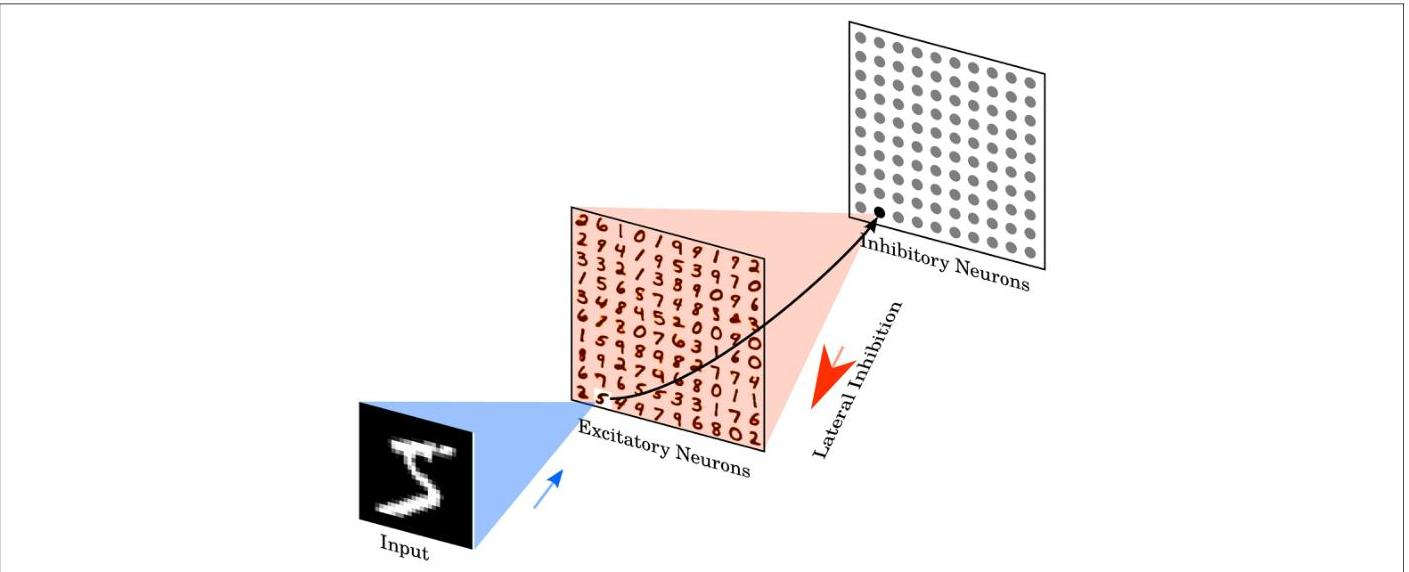
\includegraphics[scale=0.29]{snn_architecture.jpeg}
   \caption{ネットワークアーキテクチャ.28$\times$28 ピクセルの MNIST 画像の輝度値は,対応するピクセルの輝度に比例する発火率を持つポアソンスパイクに変換される.これらのポアソンスパイク列は,興奮性ニューロンへの入力として全対全方式で供給される.青色の網掛け部分は,特定の興奮性ニューロンへの入力接続を示している.興奮性ニューロンは,例のニューロンで示されているように,抑制性ニューロンと 1 対 1 で接続されている.赤色の網掛け部分は,1 つの抑制性ニューロンから興奮性ニューロンへのすべての接続を示している.各抑制性ニューロンは,接続を受け取るニューロンを除くすべての興奮性ニューロンに接続されている.クラスラベルはネットワークに提示されないため,学習は教師なし学習となる.興奮性ニューロンは,トレーニングセット全体における数字クラスへの平均応答の最高値に基づいて,トレーニング後にクラスに割り当てられる.クラスを予測するために追加のパラメータは使用されない.具体的には,SNN の上に線形分類器や同様の方法は使用されない.}
   \label{snn_architecture}
\end{figure}
ネットワークは2層で構成されている(図\ref{snn_architecture}参照).第1層は入力層で,28$\times$28個のニューロン(画像ピクセルごとに1個のニューロン)で構成されている.第2層は処理層で,可変数の興奮性ニューロンと同数の抑制性ニューロンで構成されている.各入力はポアソンスパイク列であり,第2層の興奮性ニューロンに入力される.各ニューロンのレートは,サンプル画像内の対応するピクセルの強度に比例している(セクション3.5参照).
\par
第 2 層の興奮性ニューロンは,抑制性ニューロンに 1 対 1 で接続されている.つまり,興奮性ニューロンの各スパイクは,対応する抑制性ニューロンのスパイクのトリガーになる.各抑制性ニューロンは,接続を受け取ったニューロンを除くすべての興奮性ニューロンに接続されている.この接続により側方抑制が提供され,興奮性ニューロン間の競争が発生する.抑制性シナプスから興奮性シナプスへの最大コンダクタンスは 10 nS に固定されている.ただし,正確な値はシミュレーションの結果に大きな影響を与えず,抑制性シナプスと興奮性シナプスのコンダクタンスの比率を調整して,側方抑制が弱すぎて影響がまったくなく,強すぎて勝者が選ばれると他のニューロンの発火が妨げられないようにする必要がある.
\subsection{学習}
入力ニューロンから興奮性ニューロンに至るすべてのシナプスは,STDPを用いて学習される.シミュレーション速度を向上させるため,重みのダイナミクスはシナプストレースを用いて計算される.これは,シナプス重みに加えて,各シナプスが別の値,すなわちシナプス前トレース$x_{pre}$を記録していることを意味している.$x_{pre}$は,最近のシナプス前スパイクの履歴をモデル化する.シナプス前スパイクがシナプスに到達するたびに,トレースは1増加し,そうでない場合は$x_{pre}$は指数関数的に減少する.シナプス後スパイクがシナプスに到達すると,シナプス前トレースに基づいて重みの変化$\Delta w$が計算される.
\begin{equation}
   \Delta w=\eta(x_{pre}-x_{tar})(w_{max}-w)^\mu
\end{equation}
ここで,$\eta$は学習率,$w_{max}$ は最大重み,$\mu$は更新が前の重みにどのように依存するかを決定する.$x_{tar}$ は,シナプス後スパイクの瞬間のシナプス前トレースの目標値である.目標値が高いほど,シナプス重みは低くなる.このオフセットにより,シナプス後ニューロンの発火にほとんどつながらないシナプス前ニューロンがどんどん切断されるようになる.これは,シナプス後ニューロンがめったにアクティブにならない場合に特に便利である.入力にノイズを追加し,重み減少メカニズムを学習ルールに追加して無関係な入力を切断することで,同様の効果を実現できる.ただし,このシミュレーションでは,シミュレーション時間が長くなる.学習ルールは,Querlioz らが使用したルールに似ている.しかし,ここでは時間に依存しない重みの変化よりも生物学的に妥当性の高い,指数関数的な時間依存性を使用している.
\par
選択したアーキテクチャの堅牢性を学習則の正確な形式と比較するために,他の3つのSTDP学習則をテストした.2つ目のSTDP則は,指数関数的な重み依存性を用いて次のように重みの変化を計算する.
\begin{equation}
   \Delta w=\eta_{post}(x_{pre}\exp(-\beta w)-x_{tar}\exp(-\beta(w_{max}-w)))
\end{equation}
ここで,$\beta$は重み依存性の強さを決定する.
\par
3つ目のルールは,シナプス前痕跡だけでなくシナプス後痕跡も用いるものである.シナプス後痕跡はシナプス前痕跡と同様に機能をするが,シナプス後痕跡の増加はシナプス後スパイクによって引き起こされる.さらに,この学習ルールでは,シナプス前スパイクとシナプス後スパイクの重みの変化が起こる.シナプス前スパイクの重みの変化$\Delta w$は次の通りである.
\begin{equation}
   \Delta w=-\eta_{pre}x_{post}w^\mu
\end{equation}
ここで,$\eta_{pre}$はシナプス前スパイクの学習率であり,$\mu$は重みの依存性を決定する.シナプス後スパイクの重みの変化は次の通りである.
\begin{equation}
   \Delta w=\eta_{post}(x_{pre}-x_{tar})(w_{max}-w)^\mu
\end{equation}
ここで,$\eta_{post}$は学習率,$w_{max}$は最大重み,$x_{tar}$はシナプス後スパイクの瞬間のシナプス前トレースの目標平均値である.
\par
さらに,ネットワークの重みはトリプレットSTDPルールを用いて学習した.このルールは学習に重み依存性を一切考慮しないため,ルールに重み依存性を組み込むか,他の方法で重みを制限する必要がある.ここでは,ニューロンの均等な使用を保証する除算重み正規化を使用する.
\par
べき乗則と指数的重み依存STDP則には,シナプス後興奮性ニューロンのスパイク発火時にのみ重み更新が行われるという利点がある.シナプス後ニューロンの発火率は非常に低いため,シナプス後発火に対するより複雑なSTDP更新でも多くの計算リソースを必要としない.対称学習則とトリプレット則は,シナプス前イベントごとにすべてのシナプス後ニューロンの重み変化を計算する必要があるため,ソフトウェアシミュレーションを用いたシミュレーションでは計算コストが高くなってしまう(特に大規模ネットワークの場合).
\par
\subsection{ホメオスタシス}
入力の不均一性により,興奮性ニューロンの発火頻度に差が生じ,側方抑制によりこの差はさらに大きくなる.しかし,単一のニューロンが応答パターンを支配することを防ぎ,ニューロンの受容野が確実に分化するために,すべてのニューロンの発火頻度がほぼ等しいことが望ましくなる.これを実現するために,ここでは内因性可塑性に似た適応膜閾値を採用している.具体的には,各興奮性ニューロンの膜閾値は$v_{thresh}$だけでなく,$v_{thresh}+\theta$の合計によって決定される.ここで,$\theta$はニューロンが発火するたびに増加し,指数関数的に減少する.したがって,ニューロンの発火が多いほど,その膜閾値は高くなり,その結果,ニューロンが近い将来にスパイクするためにはより多くの入力が必要になる.このメカニズムを使用すると,伝導ベースのシナプス モデルが最大膜電位を興奮性反転電位$E_{exc}$に制限するため,ニューロンの発火率が制限される.つまり,ニューロン膜閾値が$E_{exc}$(またはそれ以上)に近づくと,$\theta$が十分に減少するまでニューロンの発火頻度が低下する(または完全に発火しなくなる).
\subsection{入力エンコーディング}
ネットワークへの入力は,$0\sim9$の数字の$28\times28$ピクセル画像の60000件のトレーニング例と10000件のテスト例を含むMNISTデータセットに基づいている.入力は,MNIST 画像のピクセルの強度に比例した発火率を持つポアソン分布のスパイク列の形で,350ミリ秒間ネットワークに提示される.具体的には,最大ピクセル強度255が4で割られるため,入力発火率は$0\sim63.75$Hz になる.さらに,第 2 層の興奮性ニューロンが 350 ミリ秒以内に 5 回未満のスパイクを発火した場合,最大入力発火率は 32 Hz 増加し,画像例が再度 350 ミリ秒間表示される.このプロセスは,特定の例が表示されている間ずっと少なくとも 5 回のスパイクが発火するまで繰り返される.
\subsection{トレーニングと分類}
ネットワークを学習させるために,MNISTトレーニングセット(60000件)から画像をネットワークに提示する.新しい画像を提示する前に,150ミリ秒間入力がない状態を設け,全ニューロンの全変数が静止値(適応閾値を除く)まで減衰できるようにしておく.学習が完了したら,学習率をゼロに設定し,各ニューロンのスパイク閾値を固定する.そして,1回のトレーニングセット提示における10クラスの数字に対する最も高い応答に基づいて,各ニューロンにクラスを割り当てていく.これはラベルが使用される唯一のステップであり,シナプス重みの学習にはラベルを使用しない.
\par
クラスに割り当てられたニューロンの応答を用いて,MNISTテストセット(10000例)におけるネットワークの分類精度を測定する.予測される数字は,各ニューロンの応答をクラスごとに平均化し,平均発火率が最も高いクラスを選択することにより決定される.
\section{結果}
\begin{figure}[htbp]
   \centering
   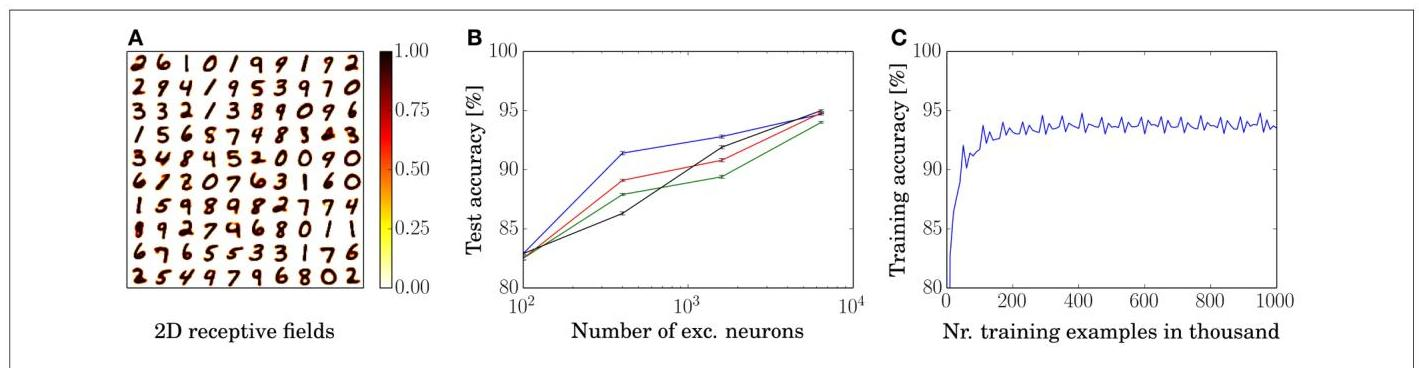
\includegraphics[scale=0.3]{snn_result1.jpeg}
   \caption{トレーニング結果.(A) $10\times10$ グリッド内の 100 個の興奮性ニューロンを持つネットワークの入力から興奮性ニューロンへの接続の重みを再配置 (784 から 28 $\times$ 28).(B) 興奮性ニューロン数の関数としてのパフォーマンス.各ドットは,学習が行われない MNIST テスト セット全体の 10 回の提示の平均として,特定のネットワーク サイズのパフォーマンスを示している.エラー バーは,テスト セットの 10 回の提示間の標準偏差を示す.各学習ルールのパフォーマンスは,それぞれ黒(べき乗法則重み依存 STDP),赤(指数重み依存 STDP),緑(事前および事後 STDP),青の線(トリプレット STDP)で示されている.(C) 提示されたトレーニング例の関数としてのトレーニング精度.最後の10000画像は,現在の10000画像のニューロンにラベルを割り当てるために使用される.例えば,画像データ30001から40000は,40001から50000を分類するためのラベルを割り当てるために使用される.これは,対称学習則を持つ1600個の興奮性ニューロンネットワークのグラフである.}
   \label{snn_result1}
\end{figure}
MNISTトレーニングセットの40000画像を用いて,100個の興奮性ニューロンを持つネットワークを学習およびテストした.その結果得られた興奮性ニューロンへの入力重みの再配置を図\ref{snn_result1}Aに示す.各ニューロンについて,784次元の入力ベクトルを28$\times$28の行列に再配置することで,ニューロンが典型的な入力を学習していることを視覚化している.
\par
100 ニューロン ネットワークに加えて,MNIST トレーニング セット全体を 3,7,15 回提示して,400,1600,6400 個の興奮性ニューロンを持つ他の 3 つのネットワークをトレーニングおよびテストした.その結果,4 つのネットワークはそれぞれ,べき乗法則の重み依存 STDP ルールで 82.9,87.0,91.9,95.0\% の平均分類精度を達成した.すべてのシミュレーションで,同じニューロン,シナプス,および STDP パラメーターを使用した(一定の応答率を維持するために適応する必要があった適応しきい値と抑制強度のパラメーターを除く).精度は,MNIST テスト セットの 10000画像を 10 回提示して平均したものである (図\ref{snn_result1}B を参照).MNIST テスト セットの強度画像はポアソン分布のスパイク列に変換されるため,スパイクのタイミングによって精度が異なる場合がある.ただし,図\ref{snn_result1}B のエラー バーに示されているように,テスト セット全体の 10 回のプレゼンテーション(同じトレーニング済みネットワークを使用)におけるパフォーマンスの標準偏差は小さく($\approx0.1\%$)なっている.
\par
残りの3つの学習ルールのパフォーマンスも図\ref{snn_result1}Bに示されている.指数関数的な重み依存性は赤で,事前・事後STDPを使用したパフォーマンスは緑で,トリプレットSTDPルールを使用したパフォーマンスは青で示されている.対称ルールを用いた1600ニューロンネットワークのトレーニング精度は図\ref{snn_result1}Cに示されている.約20万例の後,パフォーマンスは収束に近づき,100万例後でもパフォーマンスは低下せず,安定している.周期的な構造は,MNISTトレーニングセットを繰り返し提示しているためであることに注意する必要がある.この傾向は,すべてのネットワークサイズと学習ルールで同じになる.ただし,ネットワークが大きいほど,ピークパフォーマンスに達するまでのトレーニングに時間がかかる.
\begin{figure}[htbp]
   \centering
   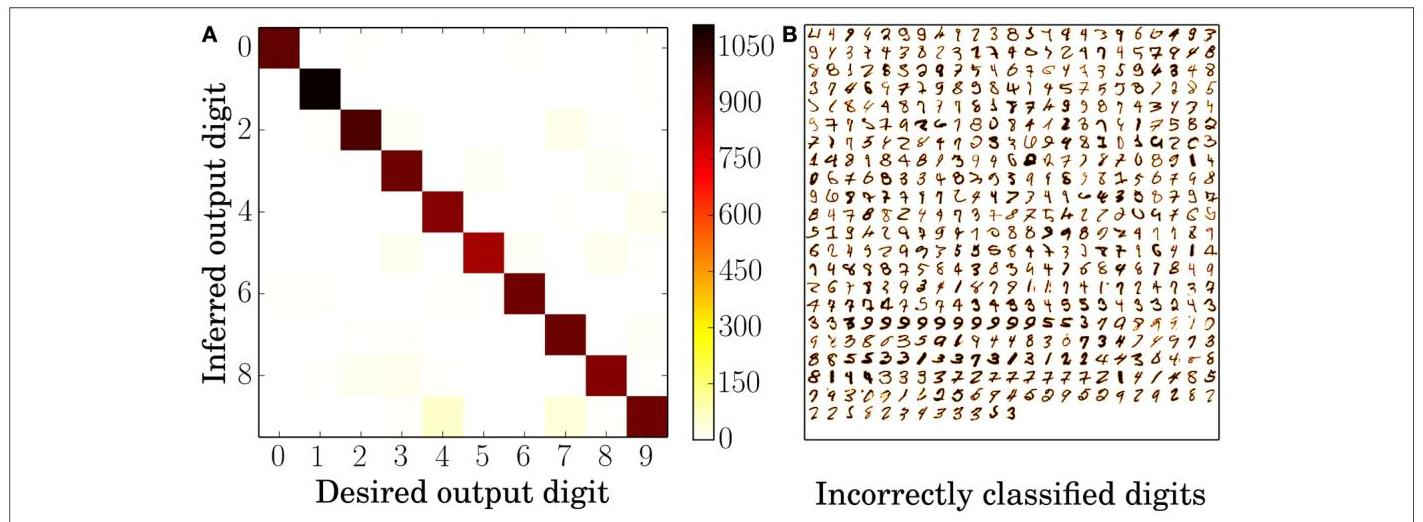
\includegraphics[scale=0.3]{snn_result2.jpeg}
   \caption{エラー分析.(A) MNISTテストセットの10000個の数字を10回提示したテスト結果の平均混同行列.同一性を示す部分で高い値を示す場合は正しく識別されたことを示し,それ以外の部分で高い値を示す場合は2つの数字(例えば4と9)の混同を示す.(B) 1つの分類で誤分類された495個の数字すべてを,MNISTテストセットの10000個の数字全体に適用した.数字のピクセルが暗いほど,その輝度値が高く,入力スパイクの頻度も高い.どちらのグラフも,標準的なSTDPルールを用いた6400個の興奮性ニューロンネットワークに基づいている.}
   \label{snn_result2}
\end{figure}
\par
標準 STDP ルールを使用した 6400 ニューロン ネットワークのエラー分析を図\ref{snn_result2}に示す.図\ref{snn_result2}A は,MNIST テスト セットの 10 回のプレゼンテーションの平均混同行列を示している.つまり,テスト例のすべての分類は 10$\times$10 のタイルのいずれかに属し,その位置は実際の数字と推定された数字によって決定される.予想どおり,分類率が 95\% であれば,ほとんどの例は正しい分類に対応する同一性上にある.より興味深いのは,誤分類された例である.最も一般的な混同は,4 が 9 として識別される回数が 57 回,7 が 9 として識別される回数が約 40 回,7 が 2 として識別される回数が約 26 回となっている.4 と 9,7 と 2 は混同されやすいが,7 が 9 と間違われることはすぐには理解できない.考えられる説明は図\ref{snn_result2}B に示されている.多くの場合,誤分類された 7 と一般的な 9 を区別する唯一の特徴は,7 の中央の水平線が上部の線に接続されていないことである.つまり,9 の受容野を持つニューロンも発火する可能性が高いということである.
\par
各ニューロンは入力数字のごく一部にしか反応しないため,応答は非常にまばらで,1つの例に対して発火するスパイクもごくわずかになる.6400個の興奮性ニューロンを持つ最大のネットワークでさえ,1つの数字の提示に対して発火するスパイクはわずか約17個である.具体的には,正しく識別された例では,同じクラスのニューロンから約16個のスパイクが発火し,異なるクラスに割り当てられたニューロンから約1個のスパイクが発火する.一方,誤って識別された例では,正しいクラスのニューロンから約3個のスパイクが発火し,他のクラスのニューロンから約12個のスパイクが発火している.

\section{考察}
\subsection{他モデルとの比較}
\begin{itemize}
   \item 教師なしSNNとしての優位性:提案したネットワークが達成した精度95\%は,教師なし学習(正解ラベルを使わない学習)を行うSNNとしては,当時報告されていた他の研究(例:Querliozらの研究で達成された93.5\%)を上回る,非常に優れた結果であった.
   \item 教師あり学習との比較と限界:一方で,この精度は,一度ANNとして教師あり学習(バックプロパゲーションなど)を行ってからSNNに変換するという,より高性能な手法(最高精度99.1\%)には及ばない.これは,生物学的妥当性を重視すると,現時点では最高の精度を出すのが難しいというトレードオフがあることを示している.
   \item 将来性:しかし,このモデルは非常にシンプルな構造(2層のみ)であるため,層を深くしてより抽象的な特徴を学習させるなどの改良によって,今後さらに性能が向上する可能性がある.
\end{itemize}
\subsection{機械学習のためのスパイクベース学習}
\begin{itemize}
   \item 最大の動機は低消費電力:SNNは,情報がスパイク(発火)という「イベント」によってのみ伝達・処理されるため,本質的に消費電力が非常に低くなる.これが,SNNを機械学習に応用する最大の動機の一つである.
   \item ニューロモーフィック・ハードウェアとの相性:この特性は,IBMのTrueNorthチップのようなニューロモーフィック・ハードウェア(脳を模倣した半導体チップ)と非常に相性が良い.これらのチップ上では,SNNはピコジュール(pJ)という極めて小さいエネルギー単位で動作させることができる.
   \item 具体的な消費電力の試算:もしこの論文で使われたネットワーク(6400ニューロン)をTrueNorthチップに実装した場合,その消費電力は1ミリワット(mW)未満に抑えられると試算されている.
   \item 応用分野:このようなスパイクベースの学習は,一度学習して終わりではなく,環境の変化に適応して継続的に学習し続ける必要があるシステム(例:ユーザーの訛りに適応する音声認識システムや,特定のセンサーに最適化される視覚システム)で特に重要になると述べている.
\end{itemize}

\end{document}